\documentclass[a4paper, 11pt]{article}
\usepackage{geometry}
\usepackage{indentfirst}
\usepackage{setspace}
\usepackage{amsmath}
\usepackage{graphicx}
\usepackage{wrapfig}
\usepackage{caption}
\usepackage{indentfirst}
\setlength{\parindent}{20pt}
\usepackage{amssymb}
\usepackage{float}

\graphicspath{ {./images/} }
\geometry{left=2.5cm, right=2.5cm, top=2.5cm, bottom=2.5cm}

\begin{document}	
	\title{Exercise \# 2. Iterative Methods For Linear Systems. }
	\author{{\small Alexandre Rodrigues (2039952)}}
	\date{\today}
	
	\maketitle
		\section*{Question 1}
			Using as a test the example usage, with $tol = 1 \times 10^{-8}$ and limiting the iterations to $maxit=250$, I got the following results. 
		
			\begin{figure}[H]
				\centering
				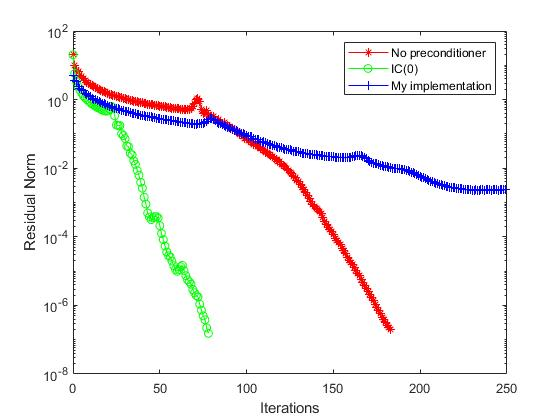
\includegraphics[width=.6\linewidth]{ex1_it250.jpg}
				\caption{Residual norm vs iteration number for PCG methods, $maxit=250$}
				\label{fig:ex1_it250}
			\end{figure}
		
			\begin{table}[H]
				\centering
				\begin{tabular}{c|c|c|c}
					\textbf{Method} 					&  \textbf{Iterations} 	& \textbf{Final Residual} 		& \textbf{Computational Time} 	\\ \hline
					Matlab PCG without preconditioning	& 			$183$ 		& $ 1.9591 \times 10^{-7} $ 	& $ 0.077 s $					\\ \hline
					Matlab PCG IC(0)					& 			$78$ 		& $ 1.5293 \times 10^{-7} $ 	& $ 0.068 s $					\\ \hline	
					My PCG implementation				& 			$250$		& $ 2.3 \times 10^{-3} $		& $	0.151 s $					\\
				\end{tabular}
				\caption{Results of PCG methods, $maxit=250$}
				\label{table:ex1_it250}
			\end{table}
		
			When $ maxit $ is large enough to guarantee convergence in all implementations we get the following results:
			\begin{figure}[H]
				\centering
				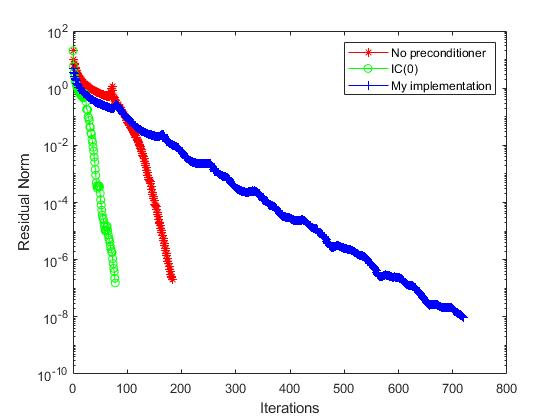
\includegraphics[width=.6\linewidth]{ex1_it750.jpg}
				\caption{Residual norm vs iteration number for PCG methods, $maxit=750$}
				\label{fig:ex1_it750}
			\end{figure}
		
			\begin{table}[H]
				\centering
				\begin{tabular}{c|c|c|c}
					\textbf{Method} 					&  \textbf{Iterations} 	& \textbf{Final Residual} 		& \textbf{Computational Time} 	\\ \hline
					Matlab PCG without preconditioning	& 			$183$ 		& $ 1.9591 \times 10^{-7} $ 	& $ 0.054 s $					\\ \hline
					Matlab PCG IC(0)					& 			$78$ 		& $ 1.5293 \times 10^{-7} $ 	& $ 0.063 s $					\\ \hline	
					My PCG implementation				& 			$720$		& $ 9.6833 \times 10^{-9} $		& $	0.351 s $					\\
				\end{tabular}
				\caption{Results of PCG methods, $maxit=750$}
				\label{table:ex1_it750}
			\end{table}
			
			My implementation is slower to converge but produces better final residual values.
			This can be explained by the simpler implementation relative to Matlab's built-in method.
			The residuals difference can derive, however, from different normalization techniques.
			
			
		\section*{Question 2}
			The spectral condition number of A is 
			
			\begin{equation}
				\kappa(A) = \frac{\lambda_{max}(A)}{\lambda_{min}(A)}.
			\end{equation}
		
			In Matlab, I used the \texttt{condest(A)} function to estimate the condition number of a sparse matrix \texttt{A}.
			
			The following table shows every data point needed to understand what the number of iterations of the CG method depends on.
		
			\begin{table}[H]
				\centering
				\begin{tabular}{c|c|c|c|c|c|c|c}
					$n_x$   & $ h $						& $\kappa(A)$			 & $ \sqrt{\kappa(A)} $& $ CG $ & $ PCG(0) $& $PCG(10^{-2})$& $PCG(10^{-3})$ \\ \hline
					$ 102 $ & $ 9.9009 \times 10^{-3} $ & $ 6.0107 \times 10^3 $ & $ 77.5288 $ 		& $ 283 $ 	& $ 87 $ 	& $ 45 $ 		& $ 17 $ 		\\ \hline
					$ 202 $ & $ 4.9751 \times 10^{-3} $ & $ 2.3810 \times 10^4 $ & $ 154.3039 $ 	& $ 532 $ 	& $ 159 $ 	& $ 78 $ 		& $ 30 $ 		\\ \hline
					$ 402 $ & $ 2.4938 \times 10^{-3} $ & $ 9.4770 \times 10^4 $ & $ 307.8473 $ 	& $ 948 $ 	& $ 282 $ 	& $ 137 $ 		& $ 53 $		\\ \hline
					$ 802 $ & $ 1.2484 \times 10^{-3} $ & $ 3.7814 \times 10^5 $ & $ 614.9304 $ 	& $ 1792 $	& $ 533 $ 	& $ 258 $ 		& $ 97 $ 		\\ 
				\end{tabular}
				\caption{Iterations of PCG methods for each value of $n_x$ and respective values of $h$ and $\kappa(A)$}
				\label{table:ex2}
			\end{table}	
		
			One can note from the table the inverse proportionality of the number of iterations on $ h = \frac{1}{n} = \frac{1}{(nx-1)} $.
			The number of iterations is halved when $n_x$ approximately doubles.		
							
		\section*{Question 3}
		
			\subsection*{Theoretical proof}
			
			One can estimate the number of iterations needed for convergence of a CG method as
			\begin{equation}
				k \approx \frac{log10}{2}p(\sqrt{\kappa}+1),
			\end{equation}
			with $tol = 10^{-p}$, so, for this example,
			\begin{align}
				k &\approx \frac{log10}{2}8(\sqrt{10^3}+1) \\
				k &\approx 300.44.		
			\end{align}
		
			This result is for a non-preconditioned method.
			
			For PCG we can find the optimal polynomial
			\begin{equation}
				P_k(t) = \left(1-\frac{t}{200}\right)\left(1-\frac{t}{400}\right)\left(1-\frac{t}{600}\right)\left(1-\frac{t}{800}\right)\left(1-\frac{t}{1000}\right)\hat{T}_{k-4}(t)
			\end{equation}
		
			This is only relevant for $t \in \lambda(A) = \{1,200,400,600,800,1000\}$.
			The error reduction is then given by the maximum value of $ \hat{T}_{k-4}(t),\ k=4,5,\ldots $.
			So the method converges when $\frac{1}{max(\hat{T}_{k-4}(t))||b||} < tol$, with $tol = 10^{-8}$ in this case.
			
			These calculations produced the following results:
			\begin{table}[H]
				\centering
				\begin{tabular}{c|c}
					\textbf{Iteration (k)} 	& \textbf{Expected Error} \\ \hline
					$4$ 					& $ 1.2 \times 10^{-3} $ 	\\ \hline	
					$5$						& $ 6.2 \times 10^{-7} $	\\ \hline
					$6$						& $ 3.1 \times 10^{-10} $	\\	\hline
					$\ldots$				& $ \ldots $	\\
				\end{tabular}
				\caption{Results for each value of implementation, no preconditioning}
				\label{table:ex3_theory}
			\end{table}
		
			It is hereby proven that the method converges after 6 iterations.		
			
			\subsection*{Testing my implementation}
			When using the Choledsky precontionier with no fill in, I did'nt get the expected results.
			Both Matlab's and my implementation converged in only one iteration.
			
			\begin{figure}[H]
				\centering
				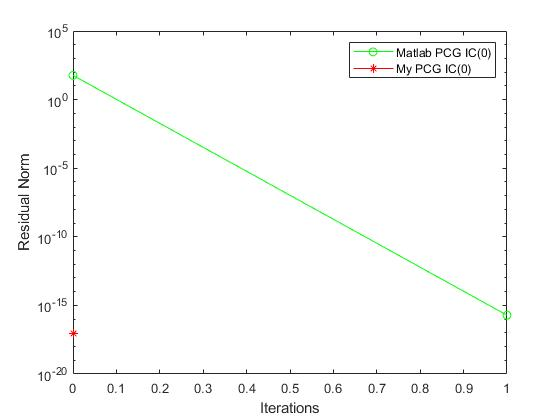
\includegraphics[width=.6\linewidth]{ex3.jpg}
				\caption{Residual norm vs iteration number for PCG methods with $IC(0)$ preconditioner}
				\label{fig:ex3}
			\end{figure}
		
			\begin{table}[H]
				\centering
				\begin{tabular}{c|c|c|c}
					\textbf{Method} &  \textbf{Iterations} 	& \textbf{Final Residual} 	& \textbf{Computational Time} 	\\ \hline
					Matlab PCG	& 			$1$ 		& $ 5.6843 \times 10^{-14} $ 	& $ 0.058 s $	\\ \hline
					My PCG		& 			$1$ 		& $ 0 $							& $ 0.020 s $	\\ 
				\end{tabular}
				\caption{Results for each preconditioned PCG implementation}
				\label{table:ex3}
			\end{table}
		
			These results can be due to the optimized preconditioner usage in this methods, making this example solved in almost only pre-processing.
			
			Due to the bad results, I tried to remove preconditioning from my implementation by setting $L$ as the identity matrix, \texttt{L = speye(size(L))}.
			\begin{figure}[H]
					\centering
					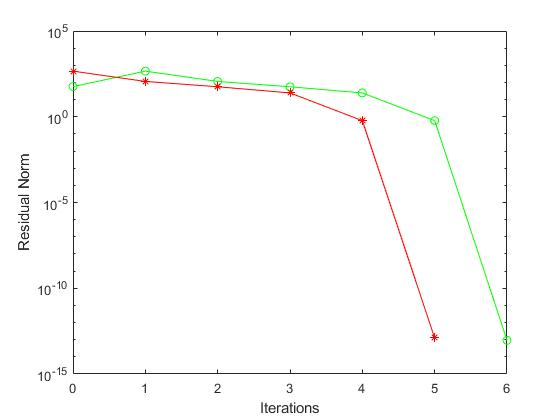
\includegraphics[width=.6\linewidth]{ex3_NoPrec.jpg}
					\caption{Residual norm vs iteration number for PCG methods without preconditioning}
					\label{fig:ex3_NoPrec}
			\end{figure}
		
			\begin{table}[H]
				\centering
				\begin{tabular}{c|c|c|c}
					\textbf{Method} &  \textbf{Iterations} 	& \textbf{Final Residual} 		& \textbf{Computational Time} 	\\ \hline
					Matlab PCG		& 			$6$ 		& $ 9.2128 \times 10^{-14} $ 	& $ 0.021 s $	\\ \hline	
					My PCG 			& 			$5$			& $ 1.2744 \times 10^{-13} $	& $	0.012 s $	\\ \hline
				\end{tabular}
				\caption{Results for each value of implementation, no preconditioning}
				\label{table:ex3_NoPrec}
			\end{table}
			These results show the theoretical calculations, my implementation is still better than expected.		
			
		
		\section*{Question 4}	
			Solving with PCG a linear system with A as the coefficient SPD matrix and b corresponding to a random vector solution, I got the following results.
				
			\begin{figure}[H]
				\centering
				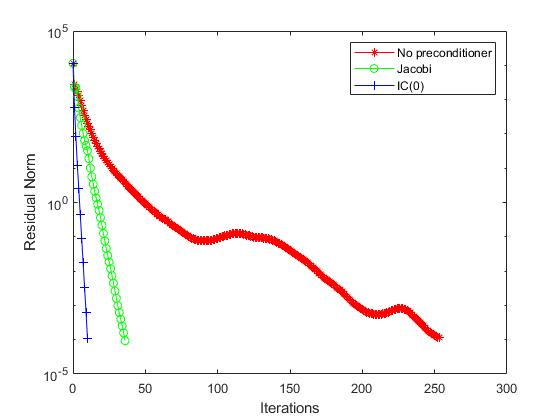
\includegraphics[width=.6\linewidth]{ex4.jpg}
				\caption{Residual norm vs iteration number for PCG methods without preconditioning}
				\label{fig:ex4}
			\end{figure}
		
			\begin{table}[H]
			\centering
			\begin{tabular}{c|c|c|c}
				\textbf{Preconditioner} &  \textbf{Iterations} 	& \textbf{Final Residual} 		& \textbf{Computational Time} 	\\ \hline
				None					& 			$253$ 		& $ 1.1367 \times 10^{-4} $ 	& $ 0.254 s $	\\ \hline
				Jacobi					& 			$36$ 		& $ 9.3198 \times 10^{-5} $ 	& $ 0.053 s $	\\ \hline		
				IC(0)					& 			$10$		& $ 1.1155 \times 10^{-4} $		& $	0.046 s $	\\
			\end{tabular}
			\caption{Results for each preconditioner}
			\label{table:ex4}
			\end{table}
		
			There is a very clear improvement when using preconditioning.
			It is also noticeable the superior characteristics of the incomplete Choledsky preconditioner relative to Jacobi.
		
		\section*{Question 5}
			Solving the linear system based on the matrix \texttt{mat13041.rig} with the GMRES method, I got the following results.
			
			\begin{figure}[H]
				\centering
				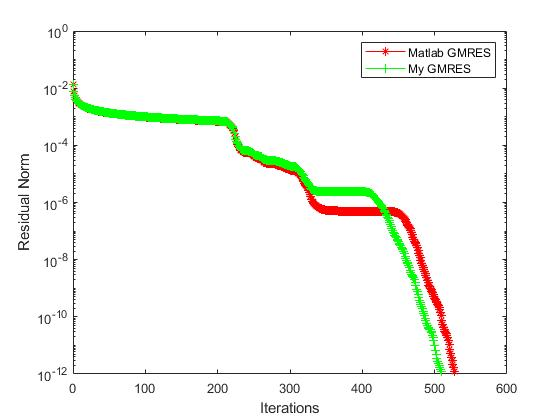
\includegraphics[width=.6\linewidth]{ex5.jpg}
				\caption{Residual norm vs iteration number for GMRES methods}
				\label{fig:ex5}
			\end{figure}
		
			\begin{table}[H]
				\centering
				\begin{tabular}{c|c|c|c}
					\textbf{Method} &  \textbf{Iterations} 	& \textbf{Final Residual} 		& \textbf{Computational Time} 	\\ \hline
					Matlab GMRES	& 			$527$ 		& $ 1.2073 \times 10^{-12} $ 	& $ 9.097 s $	\\ \hline
					My GMRES		& 			$509$ 		& $ 1.2231 \times 10^{-12} $ 	& $ 10.032 s $	\\ 
				\end{tabular}
				\caption{Results for each GMRES implementation}
				\label{table:ex5}
			\end{table}
			
			These results show that the methods have very similar convergence characteristics.
			My implementation has a smaller number of iterations but the other results are slightly worse than the ones achieved with Matlab's implementation.
					
		\section*{Question 6}
			Solving the same linear system based on the matrix \texttt{mat13041.rig} with the preconditioned GMRES method, I got the following results.
			
			\begin{figure}[H]
				\centering
				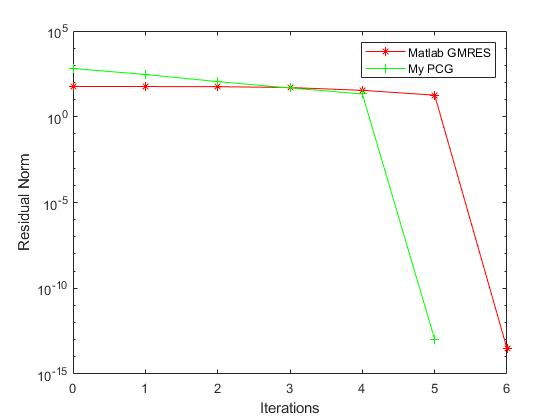
\includegraphics[width=.6\linewidth]{ex6.jpg}
				\caption{Residual norm vs iteration number for preconditioned GMRES methods}
				\label{fig:ex6}
			\end{figure}
			
			\begin{table}[H]
				\centering
				\begin{tabular}{c|c|c|c|c}
					\textbf{Method} &  \textbf{Iterations} 	& \textbf{Final Residual} 	 & \textbf{True Residual}		& \textbf{Computational Time} 	\\ \hline
					Matlab GMRES	& 			$38$ 		& $ 1.5592 \times 10^{-10} $ & $ 4.5350 \times 10^{-13} $	& $ 0.121 s $	\\ \hline
					My GMRES		& 			$39$ 		& $ 2.3797 \times 10^{-13} $ & $ 7.1893 \times 10^{-14} $	& $ 4.943 s $	\\ 
				\end{tabular}
				\caption{Results for each preconditioned GMRES implementation}
				\label{table:ex6}
			\end{table}
			
			There are clear differences in the residuals and computation time values.
			My implementation is 40 times slower but produces a true residual 5 times smaller.
			This can be due to the simplicity of my implementation and consequent unnecessary calculations.		
		
		
			Solving the linear system in 3b produced the same unexpected results as in that question.
			When using the Choledsky precontionier with no fill in both Matlab's and my implementation converged in only one iteration.
			
			\begin{table}[H]
				\centering
				\begin{tabular}{c|c|c|c}
					\textbf{Method} &  \textbf{Iterations} 	& \textbf{Final Residual} 		& \textbf{Computational Time} 	\\ \hline
					GMRES 			& 			1 			& $ 3.8481 \times 10^{-16} $	& $ 0.027 s $	\\ \hline	
					My PCG 			& 			1			& $ 1.7554 \times 10^{-17} $	& $ 0.003 s $	\\ \hline
				\end{tabular}
				\caption{Iterations for each value of nx}
				\label{table:ex6_c_prec}
			\end{table}	
		
			When I removed preconditioning form my implementation by setting $L$ as the identity matrix, \texttt{L = speye(size(L))}.
				
			\begin{table}[H]
				\centering
				\begin{tabular}{c|c|c|c}
					\textbf{Method} &  \textbf{Iterations} 	& \textbf{Final Residual} 		& \textbf{Computational Time} 	\\ \hline
					GMRES			& 			$6$ 		& $ 3.0413 \times 10^{-14} $ 	& $ 0.102 s $	\\ \hline	
					My PCG 			& 			$5$			& $ 1.0468 \times 10^{-13} $	& $ 0.012 s $	\\ \hline
				\end{tabular}
				\caption{Results for each value of implementation, no preconditioning}
				\label{table:ex6_c_NoPrec}
			\end{table}
		
			\begin{figure}[H]
				\centering
				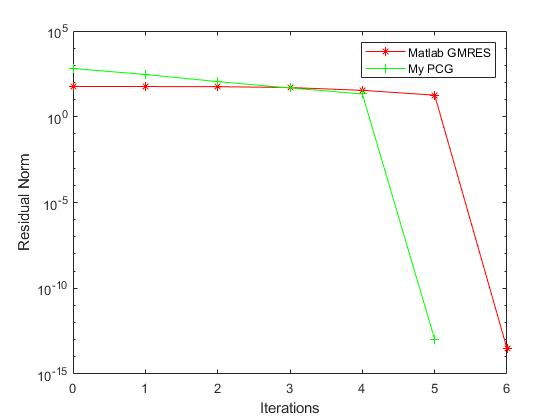
\includegraphics[width=.6\linewidth]{ex6b.jpg}
				\caption{Residual norm vs iteration number for GMRES methods without preconditioning}
				\label{fig:ex6_c_NoPrec}
			\end{figure}
		
			As in 3b, these results show the theoretical calculations, my implementation is still better than expected.				
		
		\section*{Question 7}
		
			Using the same linear system as in the previous question, we will now study the defect of the \texttt{restart} value.
			\begin{table}[H]
				\centering
				\begin{tabular}{c|c|c|c}
					\texttt{\textbf{restart}} &  \textbf{Iterations} 	& \textbf{Final Residual} 		& \textbf{Computational Time} 	\\ \hline
					$ 10 $			& 			$1149$ 		& $ 1.9901 \times 10^{-12} $ 	& $ 1.735 s $	\\ \hline	
					$ 20 $			& 			$739$		& $ 1.9741 \times 10^{-12} $	& $ 1.443 s $	\\ \hline
					$ 30 $			& 			$88$ 		& $ 1.3800 \times 10^{-12} $ 	& $ 0.242 s $	\\ \hline	
					$ 50 $			& 			$41$		& $ 9.9416 \times 10^{-13} $	& $ 0.135 s $	\\
				\end{tabular}
				\caption{Results for each value of \texttt{restart}}
				\label{table:ex7}
			\end{table}
			
			\begin{figure}[H]
				\centering
				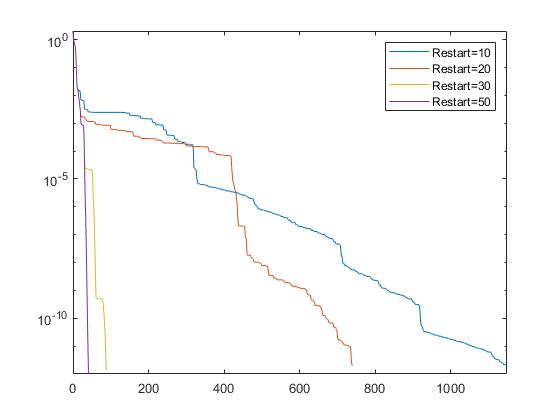
\includegraphics[width=.6\linewidth]{ex7.jpg}
				\caption{Residual norm vs iteration number for each value of \texttt{restart}}
				\label{fig:ex7}
			\end{figure}
			
			One can notice a clear improvement in convergence with the increase of the \texttt{restart} value.
			A larger \texttt{restart} value implies the method restarts less time, this is clearly better but implies a larger memory usage and computational cost.
			For \texttt{restart}$ = 50 $ the method did not restart and the results are optimal.
			This shows that this example does not benefit from restarting.
		
		\section*{Question 8}
			Solving the linear system based on the matrix \texttt{ML\_laplace.mtx} with Matlab's GMRES method, \texttt{maxit=550}, \texttt{tol=1e-8}, I got the following results.
			
			\begin{table}[H]
				\centering
				\begin{tabular}{c|c|c|c|c|c|c}
					\textbf{\texttt{droptol}} & \textbf{Iterations} & \textbf{Prec. Time}  & \textbf{Solving Time}  & \textbf{Total Time} & \textbf{Final Residual} & \textbf{$ \rho $} \\ \hline
					$2 \times 10^{-2}$ & $1316$	& $ 37.92 s $ 	& $ 44.53 s $ & $ 82.45 s $ 	& $ 5.2065 \times 10^{-7} $ & $ 0.4537 $\\ \hline
					$1 \times 10^{-2}$ & $4444$	& $ 40.55 s $ 	& $ 22.86 s $ & $ 63.42 s $ 	& $ 5.7213 \times 10^{-7} $ & $ 0.5807 $\\ \hline
					$3 \times 10^{-3}$ & $150$	& $ 51.78 s $ 	& $ 7.39 s $ & $ 59.17 s $ 		& $ 6.4998 \times 10^{-7} $ & $ 0.9401 $\\ \hline
					$1 \times 10^{-3}$ & $67$	& $ 47.74 s $ 	& $ 3.63 s $ & $ 51.37 s $ 		& $ 8.5337 \times 10^{-7} $ & $ 1.4544 $\\ \hline
					$1 \times 10^{-4}$ & $26$	& $ 43.30 s $ 	& $ 2.30 s $ & $ 45.60 s $ 		& $ 9.1517 \times 10^{-7} $ & $ 3.5140 $\\ \hline
					$1 \times 10^{-5}$ & $12$	& $ 96.73 s $ 	& $ 2.69 s $ & $ 99.42 s $ 		& $ 9.4359 \times 10^{-7} $ & $ 9.0720 $\\ \hline
				\end{tabular}
				\caption{Results for each value of \texttt{droptol}}
				\label{table:ex8}
			\end{table}
			
			\begin{figure}[H]
				\centering
				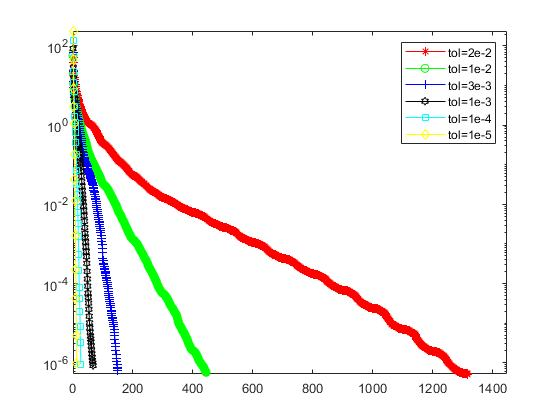
\includegraphics[width=.6\linewidth]{ex8.jpg}
				\caption{Residual norm vs iteration number for each value of \texttt{droptol}}
				\label{fig:ex8}
			\end{figure}
		
			There is a clear reduction in the number of iterations with the decrease of \texttt{droptol} which is due to the more complete factorization.
			This has a higher computational cost to compute (larger Prec. Time) but a smaller solving time.
			Despite of this, the smaller \texttt{droptol} produces a reduction in total computational time until \texttt{droptol}$ = 1\times 10^{-5}$.
			For \texttt{droptol}$  = 1\times 10^{-5} $ the Prec. time increases significantly and the solving time stagnates relative to $ 1\times 10^{-4} $.  
			The final residual does not have a noticeable change with the reduction of \texttt{droptol}.
			The density ($ \rho $) has a very clear increase with the reduction of \texttt{droptol}.			
	
\end{document}



